\documentclass[a4paper,fleqn,usenatbib]{mnras}

\usepackage{graphicx}	% Including figure files
\usepackage{amsmath}	% Advanced maths commands
\usepackage{amssymb}	% Extra maths symbols

\title[Human and machine classifications]{A transient search using combined human and machine classifications}

\author[D. Wright, C. Lintott, K. Smith et al.]{
Daryll Wright,$^{1}$\thanks{E-mail: daryll@zooniverse.org}
Chris Lintott,$^{1}$
Ken Smith,$^{2}$

$^{1}$Department of Physics, University of Oxford, Denys Wilkinson Building, Keble Road, Oxford, OX1 3RH
}

\date{Accepted XXX. Received YYY; in original form ZZZ}

\pubyear{2016}

\begin{document}
\label{firstpage}
\pagerange{\pageref{firstpage}--\pageref{lastpage}}
\maketitle

% Abstract of the paper
\begin{abstract}
Large modern surveys require efficient review of data in order to find transient sources such as supernovae, and to distinguish such sources from artefacts, noise and so on. Much effort has been put into the development of automatic algorithms, but surveys still rely on human review of targets. This paper presents an integrated system for the identification of supernovae in data from PanSTARRS, combining classifications from a citizen science project including volunteers with those from a convolutional neural network. This work represents the first time such a system has been deployed on real astronomical data, and we show that the combination of the two methods outperforms either one used individually. This result has important implications for the future development of transit searches, especially in the era of LSST and other large-throughput surveys. 
\end{abstract}

\begin{keywords}
keyword1 -- keyword2 -- keyword3
\end{keywords}

%%%%%%%%%%%%%%%%%%%%%%%%%%%%%%%%%%%%%%%%%%%%%%%%%%

%%%%%%%%%%%%%%%%% BODY OF PAPER %%%%%%%%%%%%%%%%%%

\section{Introduction}

The detection and identification of transient sources has long been an important part of astronomical observation. New surveys such as LSST (XXXXXX CITE XXXXX) will increase the number of transient candidates detected by many orders of magnitude, leading to renewed attention being paid to the methods used by transit searches. 

\section{Method}
\subsection{Pan-STARRS}
Presumably can be grabbed from elsewhere

Using data from MJD57570 and MJD 57586 for the original experiemnt, then MJD 57587 and MJD 57607 for the SVN.

\subsection{Convolutional Neural Network}

Explain how this was trained (9000 hand-labelled) 
\subsection{Citizen Science Platform}

How many people and speed 

\section{Performance}

The machine is used to identify a cutoff above which candidates are presented to human classifiers; this cutoff is chosen so that a 5\% false positive rate is acheived. This threshold involves a missed detection rate of 5.2\%. We present the results of this machine classification in figure \ref{fig:machine_dist}. A major contaminant is the presence of asteroids; they appear in the dataset as supernovae but are identified here via cross-matching with the Minor Planet Centre ephemaris database (XXXXXX). 

These data were additionally reviewed by at least one expert members of the team (normally DW or KS) to identify genuine supernovae. Candidates were divided into `real' and `bogus' categories based on these expert classifications. 

\begin{figure}
   %\vspace{200pt}
   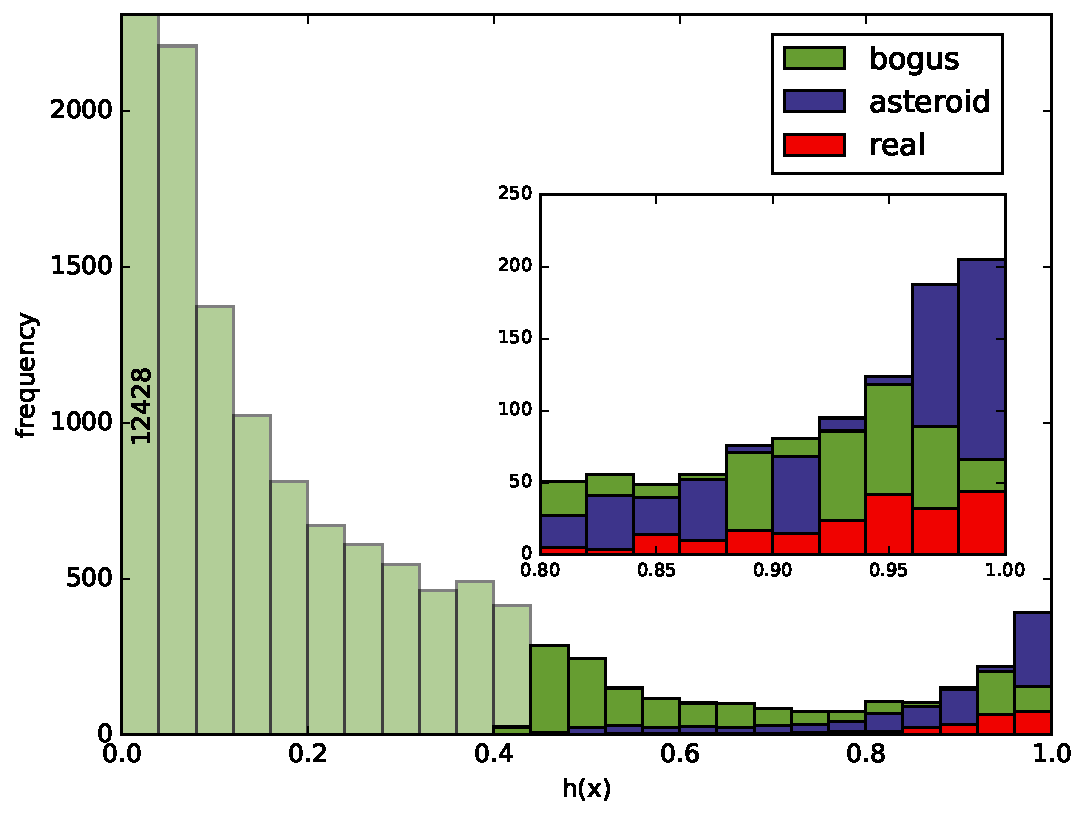
\includegraphics[width=84mm]{figs/machine_hist.pdf}
   \caption{The distribution of $P(real)$ from the current 3$\pi$ machine classifier 
            for detected objects between MJD 57570 and MJD 57586.  The light green shows the distribution of 
            objects with $P(real) < 0.436$ which are automatically rejected.  The remaining 
            objects promoted for human screening even at high values of $P(real)$ contains
            many false positives.} 
   \label{fig:machine_dist} 
\end{figure}

Candidates with high probability as assigned by the machine are more likely to be real. However, although the machine successfully rejects the majority of bogus candidates, the sample produced by the simple cut on probability is far from pure; XXXXX real candidates from XXXXXX in the sample. Higher cutoffs run the risk of rejecting an increasing number of real candidates; requiring a 1\% false positive rate will result in a missed detection rate of XXXX. 

An obvious solution to this problem is to improve the performance of the neural network, which, very broadly, is a function of the size of training set. Increasing the training set both directly improves performance but also allows for deeper, more complex networks to be built. However, it is obvious already that obtaining large, clean training sets is expensive, requiring the review of many candidates by experts. In order to reduce the burden on the science team, candidates which exceed this threshold were also classified by volunteers via the \emph{Supernova Hunters} project. The results of this analysis are shown in fig \ref{fig:human_dis}. 

\begin{figure}
   %\vspace{200pt}
   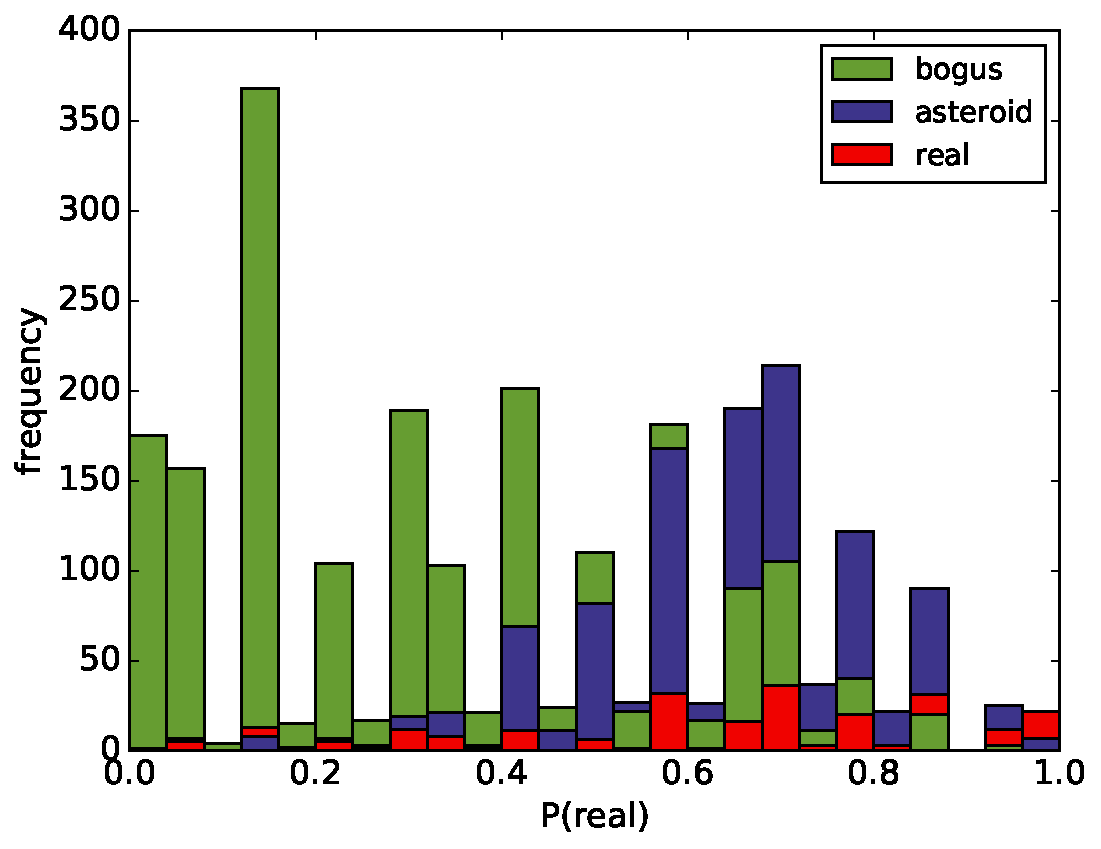
\includegraphics[width=84mm]{figs/human_hist.pdf}
   \caption{The distribution of $P(real)$ from Supernova Hunters for objects detected between 
            MJD 57570 and MJD 57586.  Compared with the machine $P(real)$ in ~\ref{fig:machine_dist}
            the objects at the extremes are pure.  There are very few real detections with 
            $P(real) < 0.04$ and few bogus detections above 0.92.} 
   \label{fig:human_dist} 
\end{figure}

\begin{figure}
   %\vspace{200pt}
   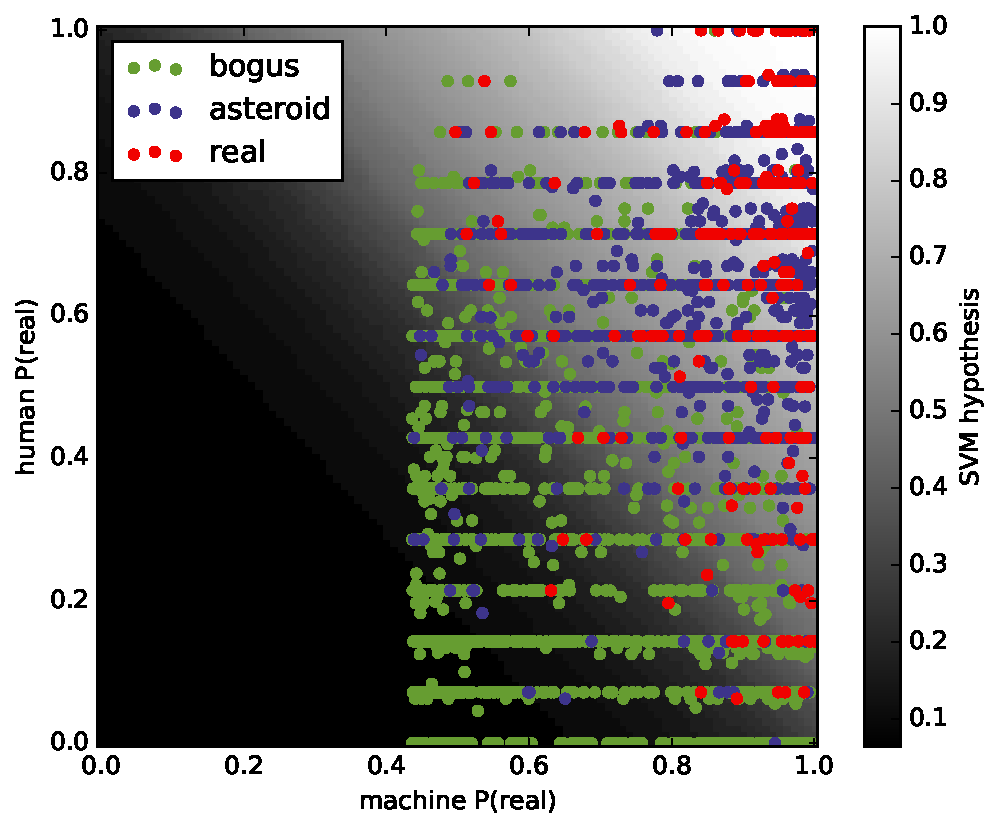
\includegraphics[width=84mm]{figs/human_v_machine_train.pdf}
   \caption{The $P(real)$ from Supernova Hunters against the machine $P(real)$ for detected 
            objects between MJD 57570 and MJD 57586.  Objects with machine $P(real) < 0.436$ are
            not uploaded to Supernova Hunters.  The background colour map shows 
            the $P(real)$ to that point in feature space by a linear SVM trained on the 
            examples shown.}
   \label{fig:combo_train} 
\end{figure}

\begin{figure}
   %\vspace{200pt}
   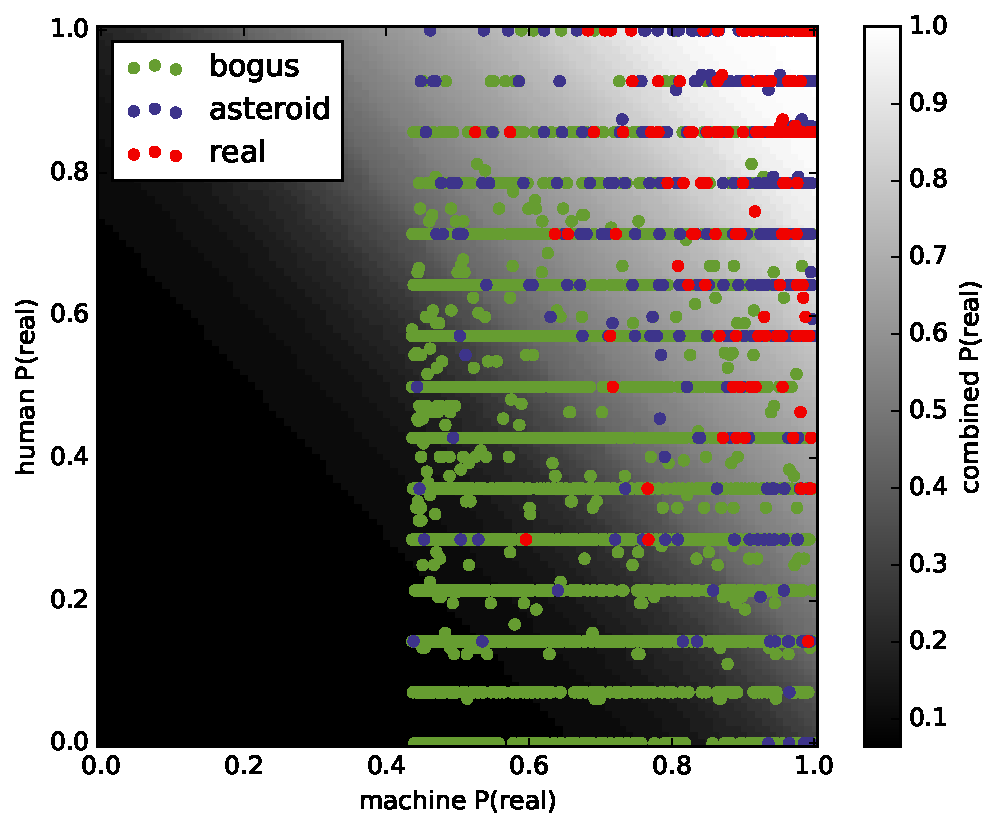
\includegraphics[width=84mm]{figs/human_v_machine_test.pdf}
   \caption{The same as ~\ref{fig:combo_train} but on a test sample of 4058 objects detected between
            MJD 57587 and MJD 57607 and held out during training of the linear SVM.} 
   \label{fig:combo_test} 
\end{figure}

\begin{figure}
   %\vspace{200pt}
   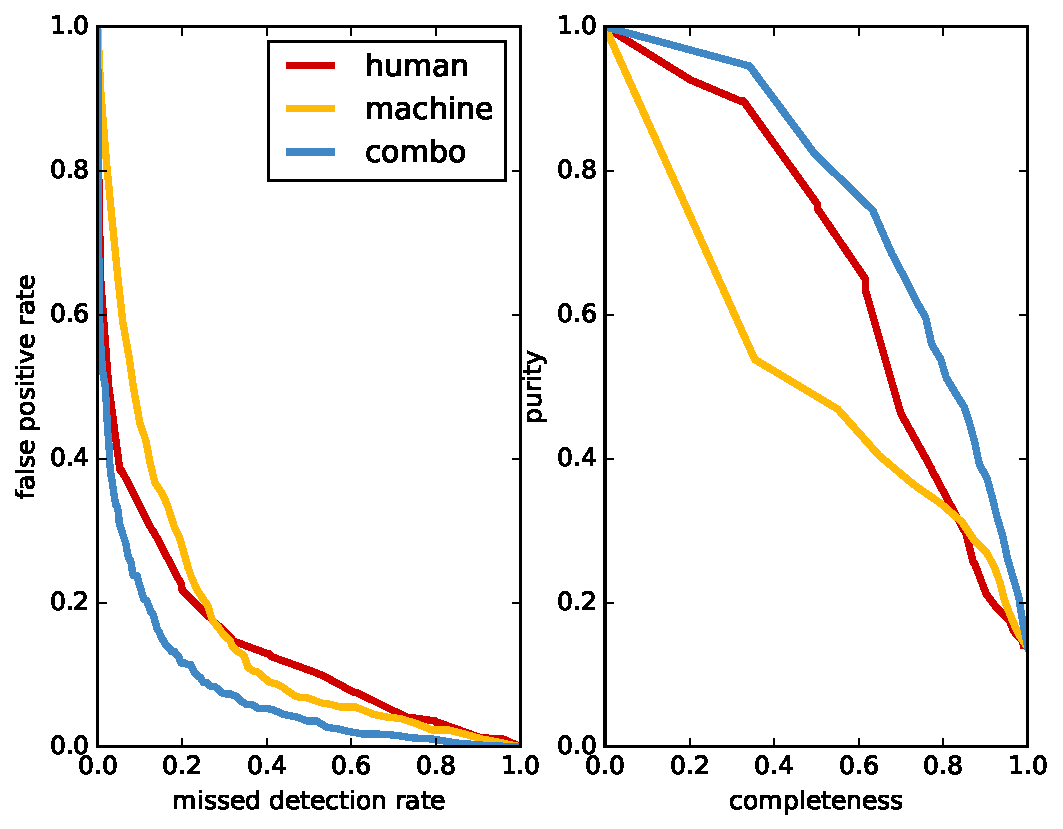
\includegraphics[width=84mm]{figs/roc.pdf}
   \caption{left: ROC curve showing performance measured on the test data in ~\ref{fig:combo_test} for human (red), machine (yellow) and
            the linear SVM combination of human and machine classifications (blue).  right: The equivalent Purity-Completeness curve.  Both
            plots show that the combination is always as good as or outperforms humans or the machine individually.} 
   \label{fig:roc} 
\end{figure}

\bsp	% typesetting comment
\label{lastpage}
\end{document}